\chapter{Case Study}
\label{ch:case}
In this chapter, we discuss the case study we conduct to validate our prototype tool, ScriptButler. The aim of the case study is to demonstrate that the functionality of the prototype tool actually helps designers analyze changes in a realistic evolution scenario. We mimic realistic evolution by taking a complex game designed by a user and removing lines of code to assess their impact. We verify the functionality of the tool with unit tests in Section \ref{sec:testing} to make sure it fulfills the functional requirements, and now we validate it to make sure that those functional requirements fulfill the goal of the tool. We first describe the case that we study, here a PuzzleScript game, and why it is useful to study it. We then explain the methodology we use when conducting our case study and what results we expect. Finally, we describe the experimental results, reflect on them, and discuss how to what extent they validate our tool.

\section{Timothy's Adventure}
The game we are studying, Timothy's Adventure\cite{timothy} has a simple concept. Steal the shiny objective, avoid the guards, and escape. You cannot escape until you have stolen the shiny objective. A sample of a level is shown in Figure \ref{fig:case_game_example}.

The victory conditions are expressed in two lines that state that the objective must have been removed and that the player must be on the "exit" tiles. The narrative of this game is that the player is a sort of thief who must grab shiny objects (represented as the objective) and exit the room (by being on the exit objects). As with most PuzzleScript games, many of its mechanics and defeat/victory conditions are implied and must be discovered by the user. Users discover either through the use of common design choices or through messages at the beginning of the level.

For this case study, we extract the exact win conditions and game mechanics by observing the code. There are five key mechanics defined by about a dozen rules. The first mechanic is tied to the \textit{Objective} Win Condition, it removes any Objective the player is adjacent to if the player presses the action key. This removes the object from being an obstacle to the first win condition. The next two mechanics relate to the defeat condition of the game. PuzzleScript does not provide the ability to create defeat conditions the same way it provides for victory conditions. By default, the defeat condition is a \emph{'softlock'}, a softlock is the act of a player progressing to a level state that cannot end with a victory. The player can still modify the level and move around (as opposed to a \emph{'hardlock'}) but will never be able to achieve victory. Sometimes, as with this particular game, the designers create explicit defeat conditions with rules that automatically restart the level if the player reaches a certain state. Two mechanics take care of this defeat condition, the first one states that if a Guard object is on the same X or Y axis as the Player object, then they will move one block in the player's direction and the second states that if a Guard is adjacent to the Player object then the Player object is replaced with another object representing that the player got "caught" and then the level restart at the next loop.

\begin{figure}[!t]
    \centering
    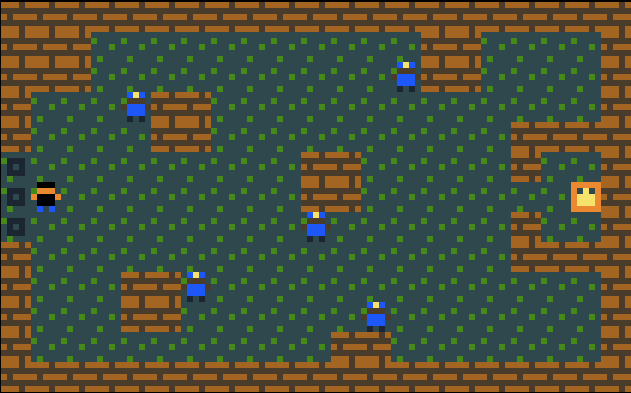
\includegraphics[width=0.75\textwidth]{images/case_results/Case_game.png}
    \caption{A level from the case game showcasing the general layout with the exit on the left, the objective on the right and the guards in blue}
    \label{fig:case_game_example}
\end{figure}

Finally, the game has two mechanics which represent tools that the player can use to solve certain levels. The first mechanic, introduced in level 5, allows the player to step on a Button object which transforms every Door object on the same X and Y axis into a different object which neither the player nor the guards can go through. This is usually used to stop guards from getting to the player but can also softlock the player if used without care. The second mechanic and the most complex one of the game is related to movement. It states that if the player steps on a Portal object, then they will be teleported to the equivalent portal object on the same X or Y axis given that it is not obstructed. This is used to allow the player to move to rooms that are not connected to one another or to escape guards as they cannot use the portal. The game contains 14 levels, each of them created with the goal of gradually increasing the difficulty by introducing new challenges and new mechanics to solve those challenges. These levels are shown in Figure \ref{fig:case_game_levels}.

\begin{figure}[!t]
    \centering
    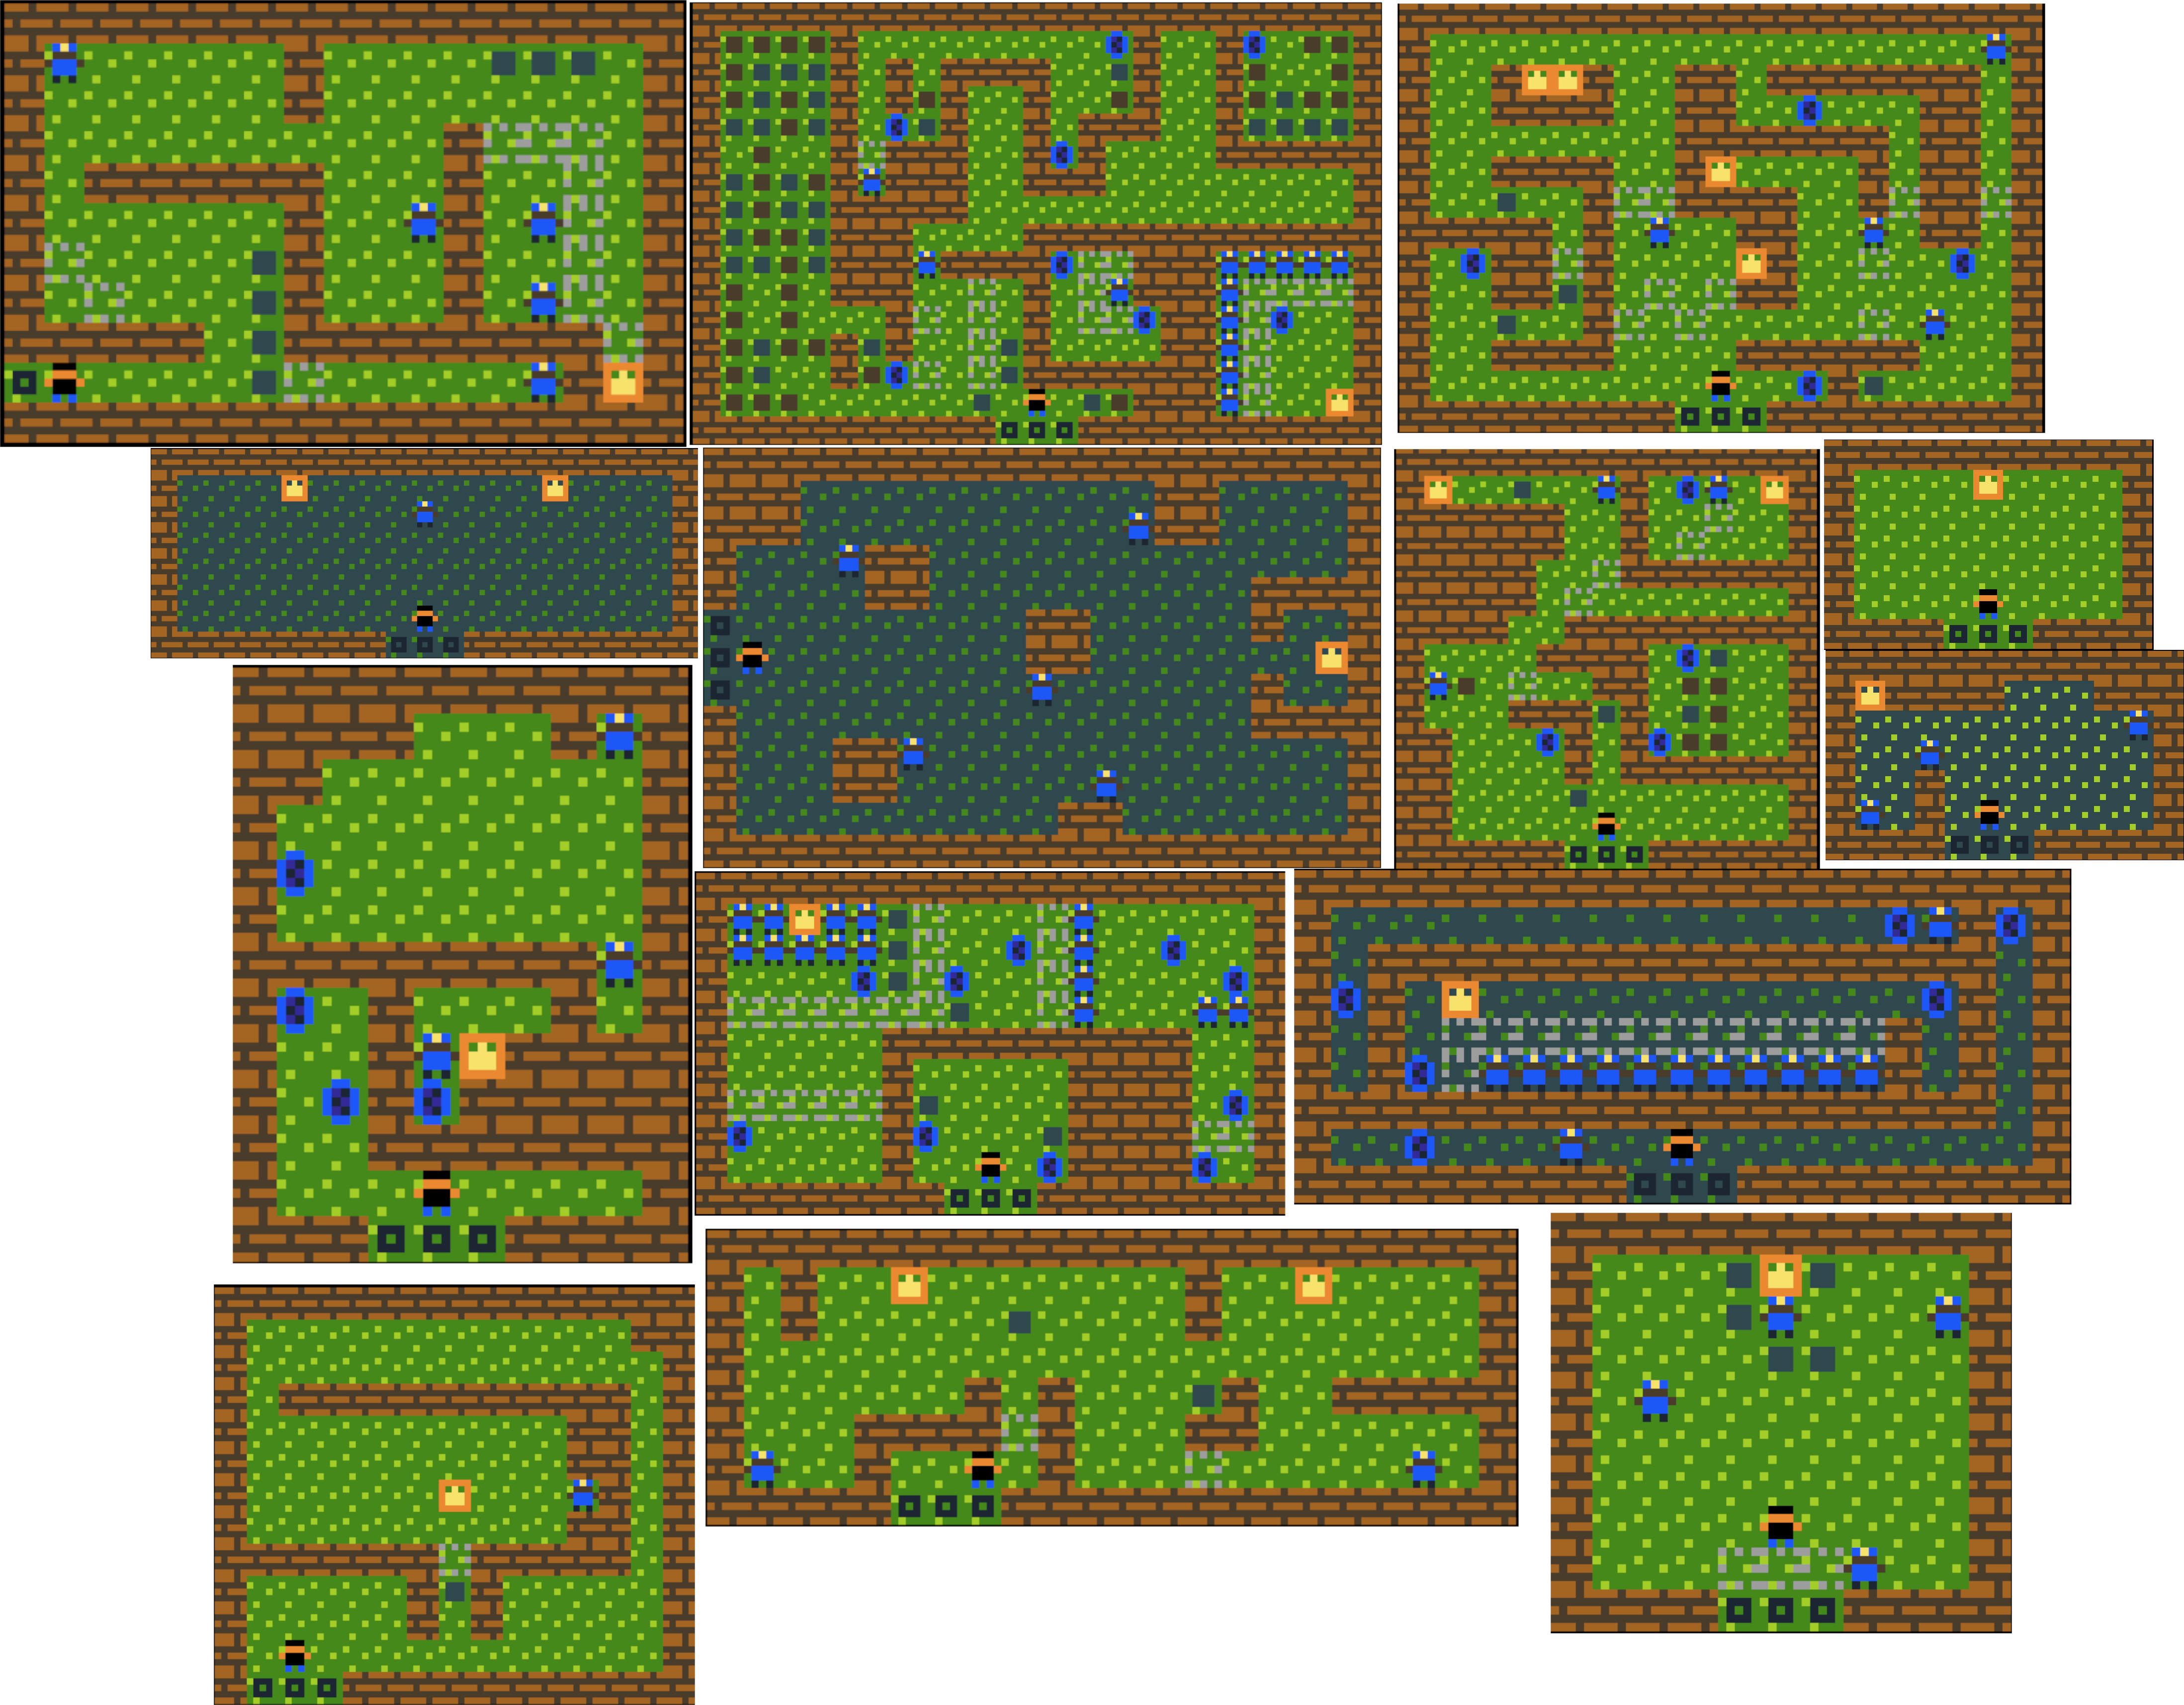
\includegraphics[width=1\textwidth]{images/case_results/Case_game_levels.png}
    \caption{A collage of all 14 levels of Timothy's Adventure}
    \label{fig:case_game_levels}
\end{figure}

\section{Approach}
This case study is based on the following hypothesis:\newline
\quad\textit{"Removing part of an existing high-quality game damages the code and gameplay in such a way that these modifications represent realistic scenarios in the evolution of that game. By studying the effects of these modifications we can learn how the game's mechanics provide affordances to the player."}

The damaged code and gameplay we refer to leaves the game technically playable. Players can still play, but their experience has been negatively impacted by the changes. The modifications we perform are intended to mimic the iterative game design. We describe selected modifications, each with a specific purpose. The modifications focus on three specific areas of a game that designers change commonly when evolving their game. We then run ScriptButler with these three modifications and observe what kind of feedback it provides. It is important that each modification is simple enough to be validated manually but complex enough to alter the gameplay in a subtle way. We also run ScriptButler on an unmodified version of the game to see what kind of issues already exist. We do not expect to find any major errors as the game runs and has been playtested by players.

Please note that we do not test our prototype tool on the published version of the game but on our own modified version, even in the case when we test on an "unmodified" version. This modified version includes additional newlines and the removal of redundant white spaces so as to make it simpler for our prototype grammar to parse it efficiently. Line numbers used in this chapter are all references to lines in our modified version which can be found on the repository of the project\footnote{\url{https://github.com/ClementJ18/ScriptButler/tree/main/src/PuzzleScript/Test/Case}}

\subsection{Victory Conditions}
The first modification is intended to study the effects of changes in victory requirements. When changing victory conditions, the difficulty of a level is impacted, either the difficulty increases (potentially to an impossible level) or it decreases (potentially to a trivial level). We create a scenario that mimics the latter by removing the Win Condition that states that no \emph{Objective} objects must be present in the level (line 210). Removing the condition removes the player's need to reach the Objective objects that are usually the main focus of a level. This alters the route they must take and since they now have fewer obstacles to overcome it lowers the difficulty of the level to a potentially trivial level. Considering the setup of the levels in the case game, we expect this change to make it possible to solve all levels by continually going in one direction.

As we described previously, the case has two Win Conditions. The second Win Condition (line 211) requires that the Player object be stacked with an Exit object to emulate the player "leaving" the room. Removing that condition does not have the same impact since the requirement is mostly focused on pathfinding. However, we can change the object that the Player needs to be stacked with to meet the condition. Therefore, our second change to the victory condition is changing the condition from being \texttt{All Player on Exit} to \texttt{All Player on Background}. This small change, which in a real scenario could happen by accident, makes it so that every level instantly meets the condition. This effect is because 'Background' objects are the default 'ground' object the player passes over when traversing the level.

Both these modifications intend to trivialize the difficulty of the game. Another realistic scenario would be making the game impossible to solve by creating a victory condition that cannot be fulfilled. We create a similar scenario in the next modification by removing a mechanic of the case. However, we can first simulate an impossible level through the creation of conflicting victory conditions\footnote{This modification is stored in Case/Modification4.PS to avoid contamination of other case files.}.

A conflicting victory condition is a result of software evolution, causing two victory conditions to be mutually exclusive. This case can occur when the mental models game designers have of their references falls out of sync. This human error can happen easily in PuzzleScript due to the fixed placement of components and the vertical space requirement pushing sections of of view easily. We simulate this scenario by adding two lines of code. The first addition is a new reference \texttt{'Object = Objective or Guardian or Exit'} (line 167). The first addition mimics a long, generic reference that game designers are more likely to forget. The second addition is a new condition (line 213) that states \texttt{'Some Object'}. The second addition mimics a victory condition that does not appear as conflicting due to naming convention but is when resolved.

\subsection{Game Mechanics}
The second modification is intended to study the effects of changes in the mechanics of the game. If the mechanics of a game change, players may no longer have the same play affordances they previously had. Some of these play affordances may have been essential to overcome the obstacles presented to the player. Therefore, the removal of the mechanic may change whether or not the player can overcome the obstacles placed in its way. We recreate that scenario by removing the rule which allows the player to remove the Objective object (line 193). Removing that rule removes one of the core mechanics of the game which is that you can "steal" the shiny objective to satisfy the victory conditions. We expect this change to make it impossible to theoretically solve this level regardless of the setup. We chose specifically this rule over others because this rule does not relate to pathfinding. ScriptButler does not currently have the capacity to evaluate rules that interact with the player's pathfinding. The rule we are removing specifically relate to the player's ability to modify their environment to meet the victory conditions. We expect the result of this modification to be the impossibility to meet the "No Objective" victory condition simply because there is no way to get from a state where there are objects present to one where there are not any present.

The modifications we have done so far impact the game in a retroactive manner. We create scenarios where the designer has an existing, working game and they change it in a way that breaks it. In the next modification, we assume that the player has a working game and existing working levels.

\subsection{Level Layout}
The third modification is intended to study the effects of evolution in level design. When level design changes, this can create new obstacles or remove certain obstacles. This kind of problem can also occur when creating new levels. We focus on how removing objects changes the required player affordances for a level and how the mechanics not meeting those requirements can actively harm the gameplay. If a level requires the player to have a crate to reach an area but the mechanics do not provide a way to get that crate then the gameplay suffers. One possibility to mimic this change is removing the Objective object from the level, but this would be very similar to the previous two modifications. As such, we instead modify the levels by removing the \emph{Exit} objects from certain levels. The expected result is that it will now be impossible to solve the level because there are no mechanics that allow the player to create Exit objects. An example of this modification is illustrated by \ref{fig:case_m3_modification}.

Creating new levels, or modifying existing ones, is a challenging task. We aim for ScriptButler to provide support for that process so game designers can avoid simple mistakes that result in bad game design. 

\section{Results}
Here we discuss the results of running and analyzing the various modifications described above with ScriptButler.

Our first test was to run the game on an unmodified version of the game, this test produced the following warnings:
\begin{itemize}
    \item WARNING: Line 33 - Color \textbf{white} not used in object Background 4
    \item WARNING: Line 161 - Legend \textbf{ + } defined but not used
    \item WARNING: Line 199 - Right side of the rule similar to rule on line 200
    \item WARNING: Line 200 - Right side of the rule similar to the rule on line 199
    \item ERROR: Line 202 - Objects in this section need to be able to stack but appear on the same layer.
\end{itemize}

We first want to address the error, a false positive as a result of a misinterpretation of PuzzleScript's design. The checker interprets the side of the rule with the error (\texttt{Background no Wall no Door\_on}) as meaning that the three items should be able to stack. However, the \emph{"no"} modifier means that none of the objects should be present for the rule to match. There is an argument to be made there that this is an unnecessary ambiguity since when objects are aligned in a part of the rule it usually means that they should be able to stack. In addition, there are already tools that can avoid this sort of ambiguity by creating an extra \textbf{or} reference that includes both, as can be seen in Figure \ref{fig:case_ambiguity}. Ultimately, however, the error is caused by the aforementioned flaws of reverse engineering as a way of reconstructing design. We encountered more of such issues and resolved by iteratively testing and updating the design of our implementation. However, because we did not test this particular case, it slipped through our checks.

\begin{figure}[!t]
\begin{lstlisting}[language=PuzzleScript]
Obstacle = Wall $\color{violet}or$ Door_on
[ $\color{violet}>$ Temp Teleport | Background $\color{violet}no$ Obstacle] $\color{BurntRed}->$ [ Teleport $\color{violet}>$ Player_stealth | Background]
\end{lstlisting}
\vspace*{-8pt}
\caption{Removing design ambiguity from the rule}
\label{fig:case_ambiguity}
\vspace*{-8pt}
\end{figure}

The remaining warnings are all valid issues with the game. They outline either dead code or potential optimizations. 

\subsection{Modifying Victory Conditions}
The first part of the modification is the removal of the 'No Objective' win condition. The results match our expectations. Upon running ScriptButler with the modification, we observed error messages relating to the fact that levels could be won by simply going in either to the left or down directions. These arrow messages can be seen in Figure \ref{fig:modification_1_results}. The error is part of our set of trivial solutions. Trivial solutions identify ways that a level could be solved that are so easy that they are considered to have a negative impact on the gameplay.

\begin{figure}[!t]
    \begin{subfigure}{1\textwidth}
        \centering
        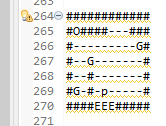
\includegraphics[scale=1.25]{images/case_results/Modification_1_Results_IDE.png}
        \caption{Game designer is notified there is an issue with this component}
    \end{subfigure}
    \begin{subfigure}{1\textwidth}
        \centering
        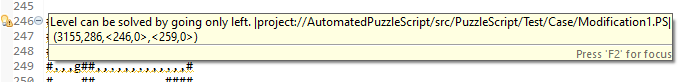
\includegraphics[scale=0.9]{images/case_results/Modification_1_Results.png}
        \caption{On hover, a message is revealed}
    \end{subfigure}
    \caption{Warning message caused by the first part of modification 1}
    \label{fig:modification_1_results}
\end{figure}

The problem we ran into with this modification is performance-related. To analyze trivial solutions, ScriptButler runs a portion of the game. Because our implementation is only a prototype the performance is not up to the user level yet. However, this performance problem does not impact the theory behind the trivial solution, minimizing its impact on validity.

The second part of the first modification is the replacement of the reference to the 'Exit' object with a reference to the 'Background' object. This change is small from a code perspective, it only modifies one reference, but has a large impact. This demonstrates how ScripButler can assist game designers in cases where they make simple errors with big consequences. The results of this modification can be seen in Figure \ref{fig:modification_1_results_part2}. The warning is raised because all objects exist on top of a Background object by default, and since we remove the other victory condition then the player can achieve victory without moving. If we add the 'Objective' victory condition back in, the warning simply alerts us that the modified condition is already met but that the level itself still needs player interaction. The other message that can be seen in Figure \ref{fig:modification_1_results_part2} represents the basic metrics that the tool displays for the convenience of the game designer. The tool does not interpret those metrics but rather displays them raw for the game designer to draw their own conclusion. The reasoning behind this choice is that interpreting metrics is non-trivial and falls outside the scope of this project. 

\begin{figure}[!t]
    \begin{subfigure}{1\textwidth}
        \centering
        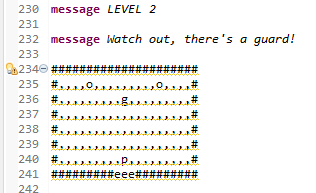
\includegraphics[scale=1.25]{images/case_results/Modification_1_Results_part2_IDE.png}
        \caption{Game designer is notified there is an issue with this component}
    \end{subfigure}
    \begin{subfigure}{1\textwidth}
        \centering
        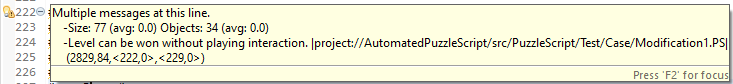
\includegraphics[scale=0.9]{images/case_results/Modification_1_Results_part2.png}
        \caption{On hover, a message is revealed}
    \end{subfigure}
    \caption{Warning messages caused by the second part of modification 1}
    \label{fig:modification_1_results_part2}
\end{figure}

Modifying victory conditions is not the most common of evolution. A victory condition is usually tied very closely to the narrative the game designers create. It is more common for the levels and game mechanics to change. However, modifying victory conditions is still a valid example of game evolution and of its impacts on gameplay. Our tool generates error messages that aim to inform the game designer of the impact of their changes on the difficulty of their level. Game designers that use ScriptButler do not have to playtest their games after changing victory conditions in cases where the changes make certain levels impossible or trivial. Instead, the tool directly informs them and gives them the chance to adjust the code to better meet their design.

\begin{figure}[!t]
    \begin{subfigure}{1\textwidth}
        \centering
        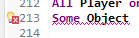
\includegraphics[scale=1.25]{images/case_results/Modification_1_Results_part3_IDE.png}
        \caption{Game designer is notified there is an issue with this component}
    \end{subfigure}
    \begin{subfigure}{1\textwidth}
        \centering
        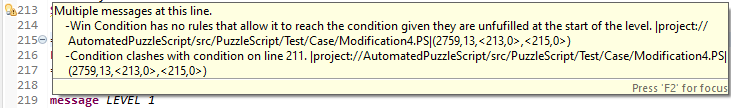
\includegraphics[scale=0.9]{images/case_results/Modification_1_Results_part3.png}
        \caption{On hover, a message is revealed}
    \end{subfigure}
    \caption{Warning messages caused by the third part of modification 1}
    \label{fig:modification_1_results_part3}
\end{figure}

Finally, Figure \ref{fig:modification_1_results_part3} shows the results of the third part of modification 1. The third part was the addition of a new reference and victory condition, resulting in mutually exclusive conditions. The results match our expectations. ScriptButler informs the game designer that the conditions are mutually exclusive making the levels unwinnable. This change focuses on showing how ScriptButler can support human developers when they make human errors. The tool does not only support developers that make design decisions with negative impacts but also those that make code decisions with negative impacts. Additionally, this part of the modification also generates another message because there are not game mechanics that support fulfilling it. We discuss these kinds of issues further in the next section. 

\subsection{Modifying Game Mechanics}
The second modification is the removal of the rule use to remove 'Objective' objects from a level. The results of the second modification match our expectations. Running our prototype with the modification generates warnings next to the 'No Objective' win condition. These warnings state that, assuming the condition to be false at the beginning of a level, there is no way for the condition to become true. These messages can be seen in Figure \ref{fig:modification_2_results}. ScriptButler achieves this by analyzing the rules and seeing if there are any potential chains that lead from the object being present to the object no longer being present.

\begin{figure}[!t]
    \begin{subfigure}{1\textwidth}
        \centering
        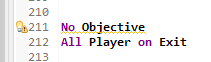
\includegraphics[scale=1.25]{images/case_results/Modification_2_Results_IDE.png}
        \caption{Game designer is notified there is an issue with this component}
    \end{subfigure}
    \begin{subfigure}{1\textwidth}
        \centering
        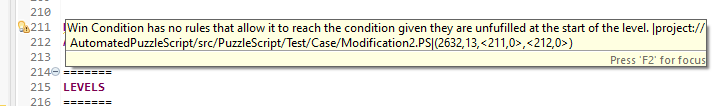
\includegraphics[scale=0.9]{images/case_results/Modification_2_Results.png}
        \caption{On hover, a message is revealed}
    \end{subfigure}

    \caption{Warning message caused by modification 2}
    \label{fig:modification_2_results}
\end{figure}

In this modification, ScriptButler presents the game designer with a complex problem. The tool does the tedious work of figuring out if there is a problem, but it does not offer a solution. Game designer need to have the necessary knowledge to deal with each message. In addition, game designers will also have a learning curve related to deciphering the meaning of the messages. However, this curve can be softened in future works studying the wording of the messages. Since they are centralized, changing the wording is a trivial task. 

Suggesting a solution to each problem is nontrivial as the error can reside in different areas. For instance, in this case, the error can be with either the WinCondition or the Rules. Part of the solution could be simply stating that fact. If the game designer knows where to place their solution they are more likely to find a fix. We do this partially by placing the message near the problematic line. Another possibility is suggesting game mechanics that could potentially fix the issue. The tool can be used to test various fragments of code that could then be suggested to the user. This solution relates more to the realm of PCG and as such, is left as future work. 

\subsection{Modifying Level Layouts}
The final modification is the remove of 'Exit' Objects from certain levels. The results of the third modification match our expectations. It is a bit trickier than we initially intended because of the \emph{Player} object mentioned in the victory condition. This object has a set of "built-in" rules that are part of the PuzzleScript engine relating to movement. We add an exception to the rules to prevent this issue from occurring. With the issue resolved, ScriptButler checks different rule chains in an attempt to see if any results in an Exit object spawning. As expected, the tool does not find any chain that meets the requirement and as such displays an error message next to the problematic levels as can be seen in Figure \ref{fig:modification_3_results}.

\begin{figure}[!t]
    \begin{subfigure}{1\textwidth}
        \centering
        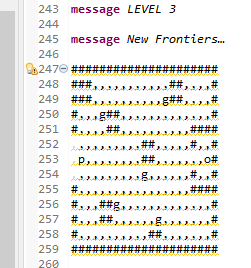
\includegraphics[scale=1.25]{images/case_results/Modification_3_Results_IDE.png}
        \caption{Game designer is notified there is an issue with this component}
    \end{subfigure}
    \begin{subfigure}{1\textwidth}
        \centering
        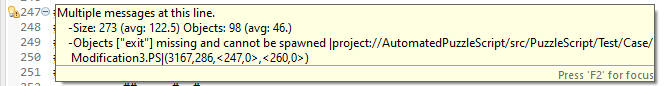
\includegraphics[scale=0.9]{images/case_results/Modification_3_Results.png}
        \caption{On hover, a message is revealed}
    \end{subfigure}
    \caption{Warning messages caused by modification 3}
    \label{fig:modification_3_results}
\end{figure}

\begin{figure}[!t]
\begin{lstlisting}[language=PuzzleScript]
(BEFORE)
###########
#....O....#
#.........#
#.........#
#.........#
#....P....#
####EEE####

(AFTER)
###########
#....O....#
#.........#
#.........#
#.........#
#....P....#
####...####
\end{lstlisting}
\vspace*{-8pt}
\caption{Removing exit objects from level}
\label{fig:case_m3_modification}
\vspace*{-8pt}
\end{figure}

We validate this check by temporarily adding a rule to the modification that would allow the player to spawn an exit. This successfully erases all error messages relating to that issue and confirms that the tool works as intended. By conducting this test, we showcase how ScriptButler can be used to support game designers in creating levels. ScriptButler warns the designer when they create levels that are impossible to solve. However, we always assume that this impossibility comes from mechanics rather than pathfinding. 

\section{Conclusion}
In our case study, we have demonstrated that ScriptButler can empower designers in realistic evolution scenarios. Using ScriptButler level designers can study the effects of any change on the code quality, and reason about the effects on gameplay. Being able to detect these changes without manually playtesting should help the game designers focus the playtesting on the more complex areas of gameplay. ScriptButler's extensible nature leads us to believe that a similar approach could be applied to many other scenarios. The tool cannot currently detect changes that affect the quality of a gameplay from a pathfinding perspective. Changes that impact alter pathfinding obstacles and impact player movement are not detected in a meaningful way. However, there is potential for pathfinding algorithms to be implemented to allow for automated testing of solutions. 

Ultimately, ScriptButler generates error messages that bring potentially harmful changes to the designer's attention. These errors are detected continuously as the design programs their game. This live feedback increases the efficiency of designers and reduces the time consumed by playtesting by reducing the need for playtesting. The extensible nature of the tool allows designers to fine tune the analysis to their specific project.
